%!TEX root = ./lec03_hardware.tex

\begin{frame}

\begin{block}{definition}
An \textbf{operating system (OS)} is system software that manages computer hardware, software resources, and provides common services for computer programs.\footnotemark
\end{block}

\footnotetext{\url{https://en.wikipedia.org/wiki/Operating_system}}

\vskip1em

The OS is responsible for ensuring that applications don't interfere with one another and that all applications and users have a fair share of the computing resources.

To do that, the OS acts as the arbiter that gives and takes access to resources, as needed.

\end{frame}

\begin{frame}

In a modern multi-tasking OS, each application is executed by one or more \textbf{processes}. 

\begin{center}
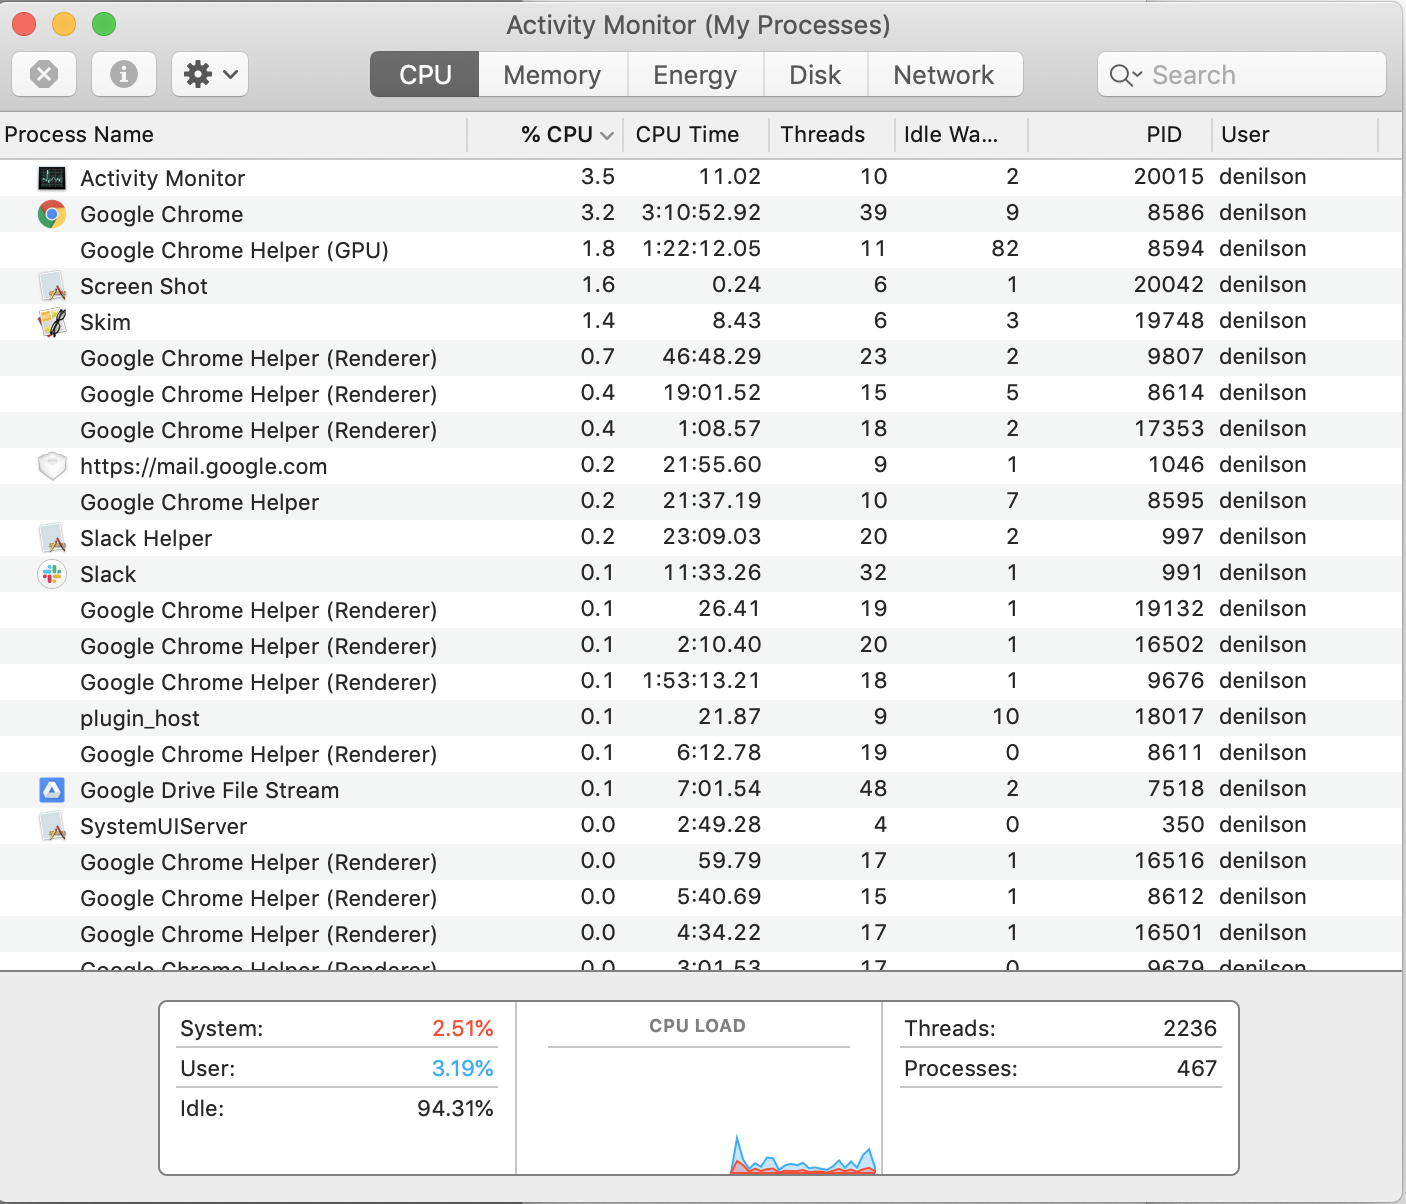
\includegraphics[width=0.75\textwidth]{figures/Activity_Monitor.png}
\end{center}

\end{frame}

\begin{frame}

Processes cannot interfere with one another, meaning:
\begin{itemize}[-, noitemsep]
\item Each user process has its own (virtual) memory buffers and its own files.
\item No process can read/write buffers (and files) ``owned'' by another user/application.
\end{itemize}

\vskip2em

The OS, however, can swap (in/out) data memory buffers of any process as needed.

\vskip1em 

The OS gives the \alert{illusion of real time parallel execution} of multiple processes by constantly swapping processes in/out of the CPU.

\end{frame}


\begin{frame}

What does this have to do with databases?

A DBMS is a complex application, that is implemented by \textbf{many} processes:
\begin{itemize}[-, noitemsep]
\item In some systems, each user query is executed by a separate OS process (normally owned by the same OS user).
\item Often, there will be processes for each user connection in a multi-user system.
\item At least, each large module of the DBMS is implemented by a different process (e.g., query processing, backups, logging, indexing, ...).
\end{itemize}
\end{frame}

\begin{frame}

Over-simplified view of the various OS processes comprising a DBMS:


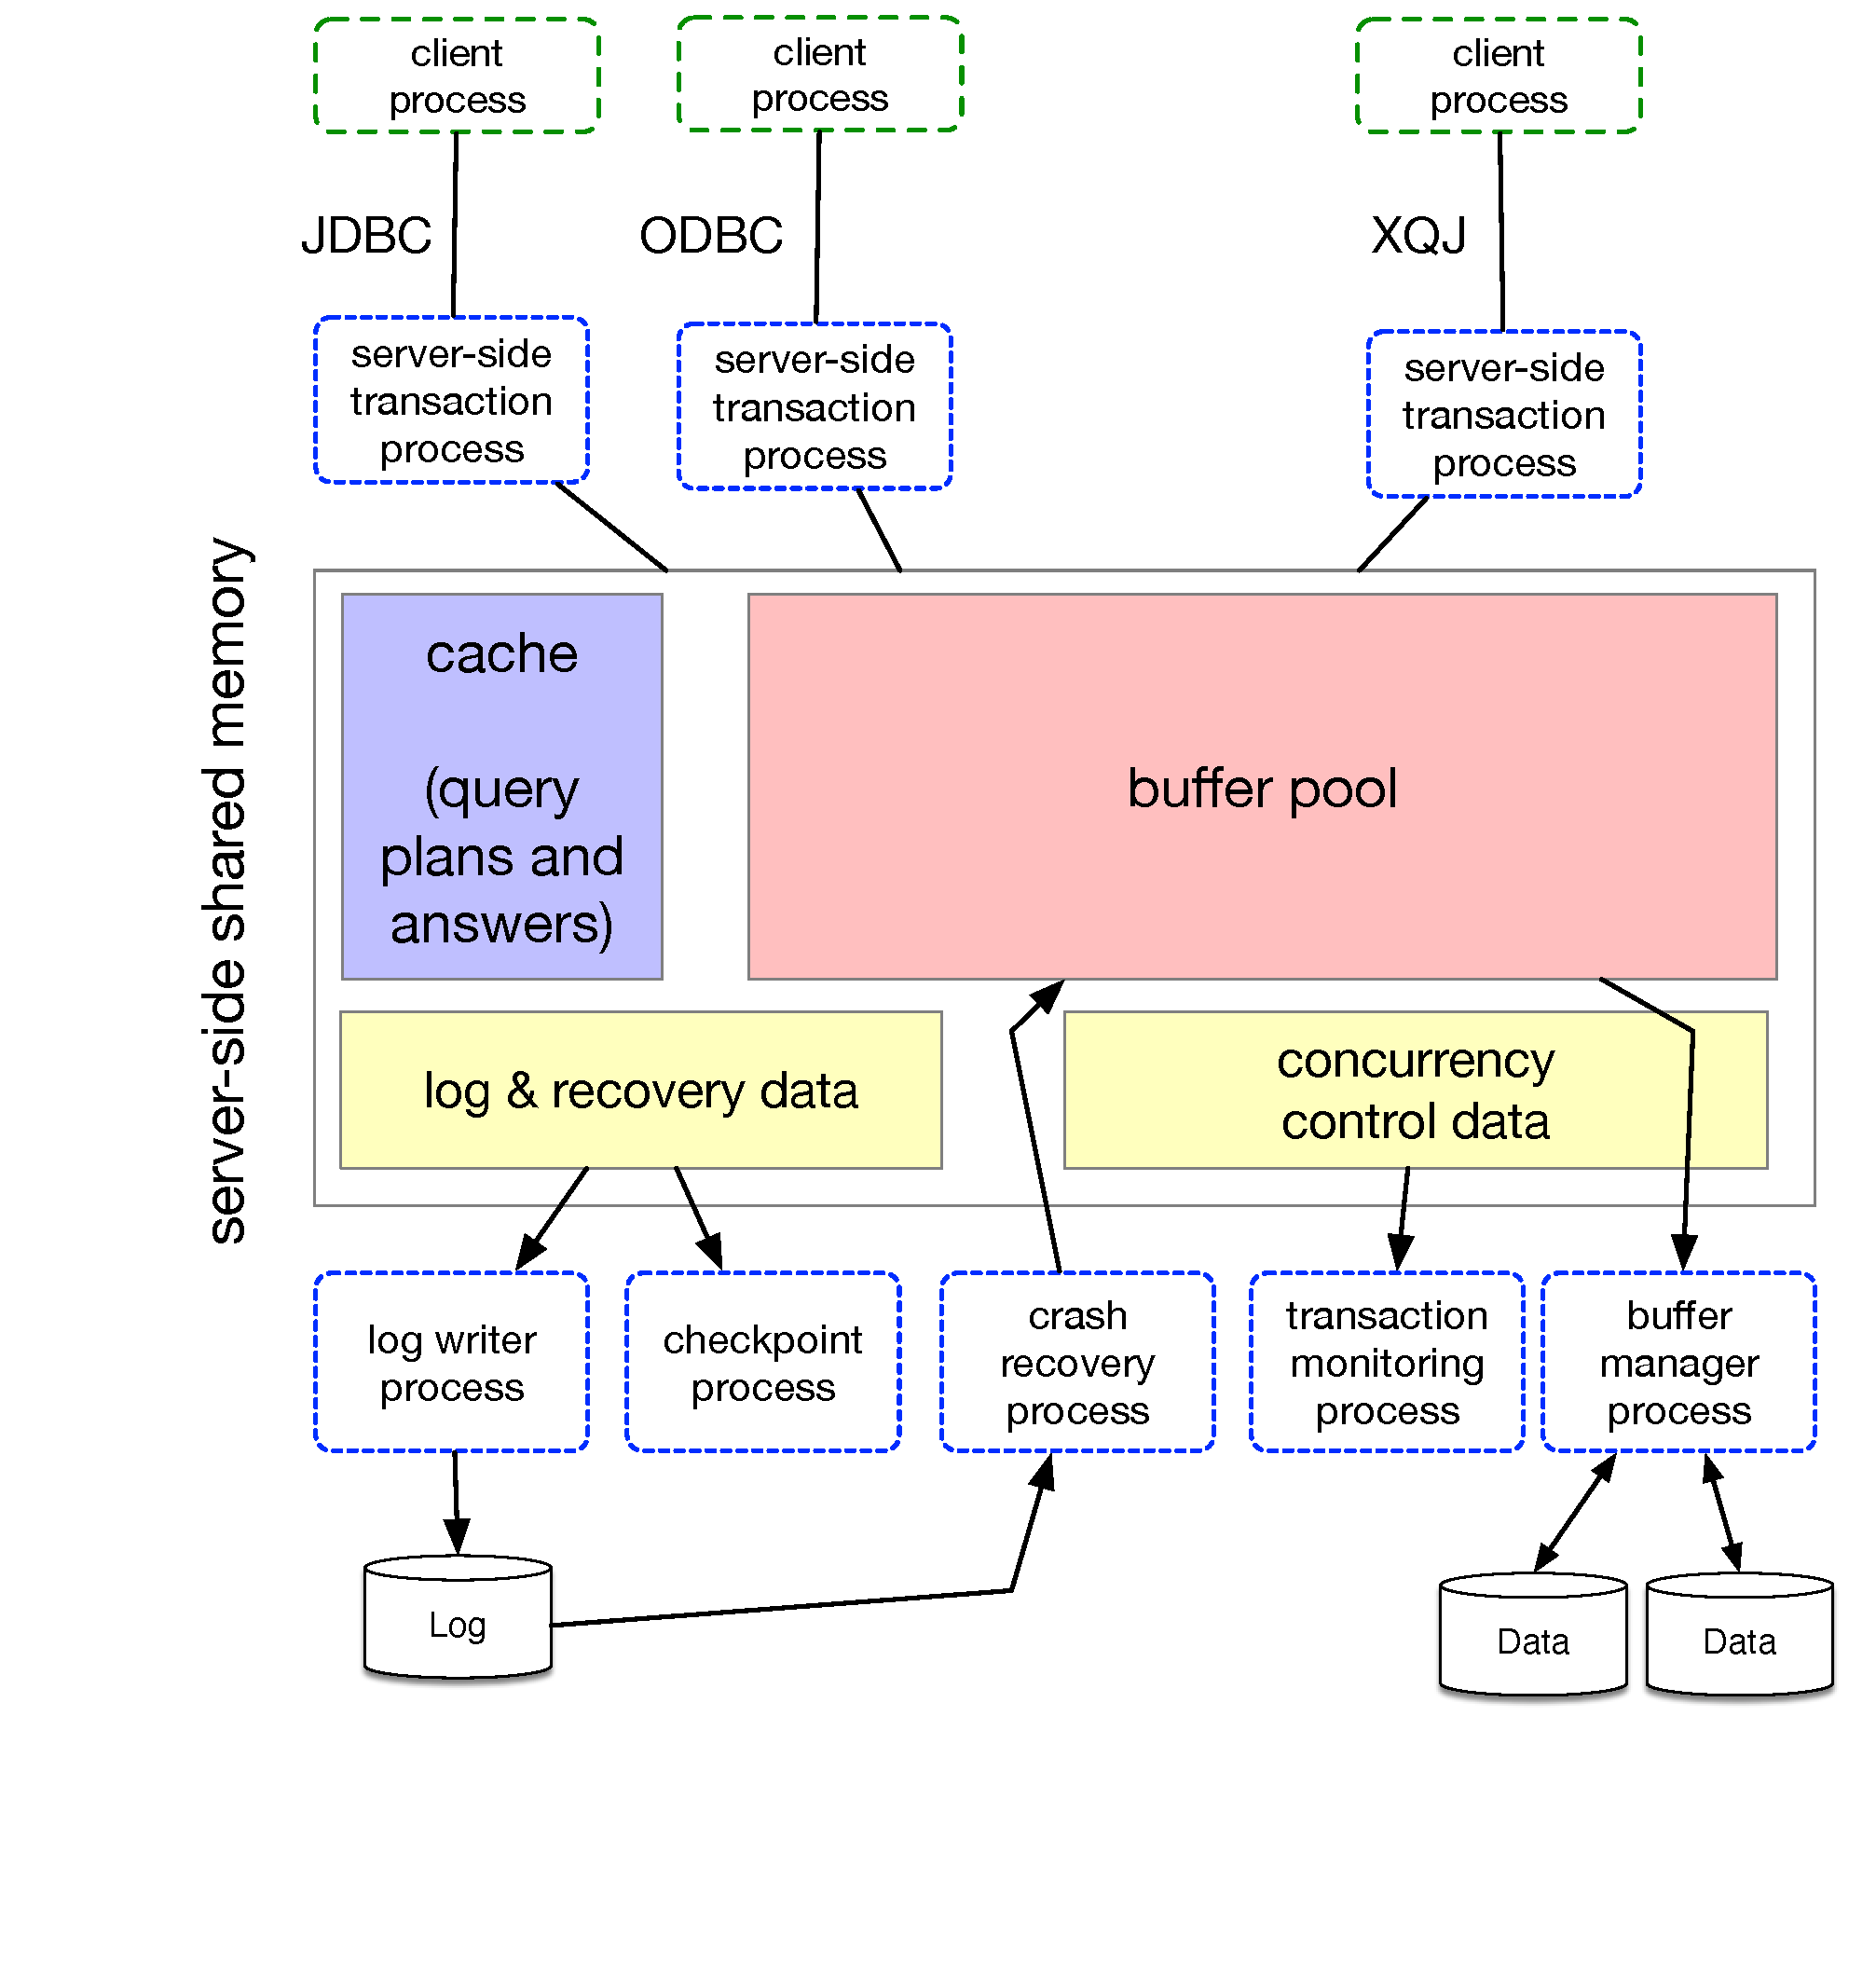
\includegraphics[width=0.8\textwidth]{figures/processes_memory_disks.eps}

\end{frame}
